\documentclass{beamer}

% Used packages

\usepackage[czech]{babel}
\usepackage[utf8]{inputenc}
\usepackage{multirow}
\usepackage{graphicx}
\usepackage{amsmath,bm,times}
\usepackage{tikz}
\usepackage{verbatim}
\usepackage{listings}
\usepackage{color}
\usepackage[ruled,noline]{algorithm2e}

\useoutertheme{infolines}
\usetheme{Copenhagen}
\mode<presentation>

\newcommand{\inabox}[2]{\tikz[baseline]{\node[rectangle,anchor=base,minimum
height=4mm,fill=#1] {#2};}}

% informace pouzite pro titulky

\title[Rozhodovací procedura pro logiku WS$k$S]{Rozhodovací procedura pro logiku
WS$k$S}
\subtitle{EEICT}
\author[T. Fiedor]{bc. Tomáš Fiedor}
\date{24. květen 2014}
\institute[vedoucí: Lengál]{pod vedením Ing. Ondřeje Lengála}

\begin{document}

\setbeamertemplate{footline}[infolines theme]

  \begin{frame}[plain]
    \titlepage
  \end{frame}

  \begin{frame}{Proč se vůbec zabývat logikami?}
  \begin{figure}
  \begin{center}
   \scalebox{0.5}{\includegraphics{Susanne}}
   \caption{Převzato z: Presentation for Seminar on Decision Procedures.
   \emph{Susanne Van Den Elsen}}
   \end{center}
   \end{figure}
  \end{frame}	

	\begin{frame}{WS$k$S logika}
     \begin{itemize}
       \item WS$k$S je logika
       \begin{itemize}
         \pause
         \item {\color{blue}{druhého řádu}} $\Rightarrow$ možnost kvantifikace
         přes relace;
         \pause
         \item {\color{blue}{monadická}} $\Rightarrow$ relace jsou unární, tzn.
         množiny a nikoliv např. funkce;
         \pause
         \item {\color{blue}{slabá}} $\Rightarrow$ tyto množiny jsou konečné;
         \pause
         \item {\color{blue}{s $k$ následníky}} $\Rightarrow$ možnost vyjádření
         stromových struktur.
         \pause
       \end{itemize}
              \item Příklad formule: $\varphi \overset{\mathit{def}}{=}
    \neg\exists P:
    Singleton(P) \wedge P
    \not\subseteq X$
       \pause
       \item Sémantika:
        \begin{itemize}
          \item Kódování množin jako binarní řetězce: $\{1, 3, 5\} = 010101$
        \end{itemize}
        \pause
       \item Příklady reálného využití WS$k$S:
       \begin{itemize}
         \item zpracování a verifikace jazyka,
         \item syntéza kontrolerů,
         \item integrace v Theorem Proverech,
         \item verifikace Hardware, protokolů, programů.
       \end{itemize}
     \end{itemize}
	\end{frame}
  
  \begin{frame}[t]{Rozhodování WS$k$S pomocí DFA}
  \begin{enumerate}
    \item[] Mějme formuli $\varphi \overset{\mathit{def}}{=}
    {\color<5,6>{red}\neg{\color<4>{red}\exists P:
    {\color<3>{red}{\color<2>{red}Singleton(P)} \wedge {\color<2>{red}P
    \not\subseteq X}}}}$
    \setcounter{enumi}{0}
    \only<2>{\item Konstrukce automatů korespondujících atomickým formulím
    $Singleton(P)$ a $P \not\subseteq X$}
    \setcounter{enumi}{1}
    \only<3>{\item Konstrukce průniku automatů}
    \setcounter{enumi}{2}
    \only<4>{\item Projekce automatu nad stopou odpovídající proměnné $P$}
    \setcounter{enumi}{3}
    \only<5,6>{\item Konstrukce komplementu automatu
    \begin{enumerate}
      \only<5>{\item Determinizace automatu}
    \setcounter{enumii}{1}
      \only<6>{\item Prohození koncových a nekoncových stavů}
    \end{enumerate}}
    \setcounter{enumi}{4}
    \only<7>{\item Formule $\varphi$ je platná právě tehdy když jazyk automatu
    $\mathcal{A}_\varphi$ $L(\mathcal{A}_\varphi)$ je universum}
  \end{enumerate}
  \begin{figure}
 \begin{center}
  \only<2>{\scalebox{0.55}{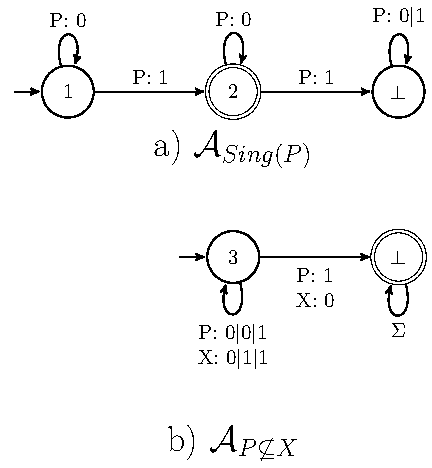
\includegraphics{formula-singleton-and-subset.pdf}}}
  \only<3>{\scalebox{0.55}{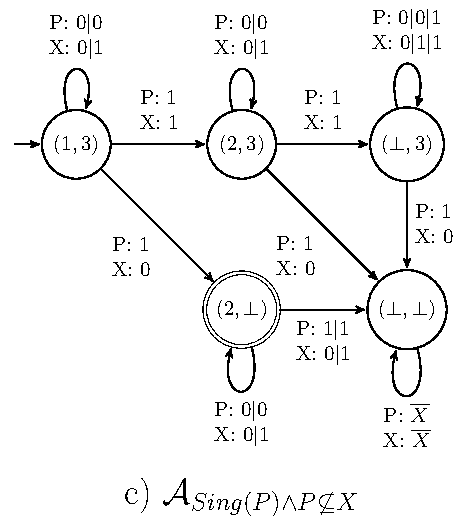
\includegraphics{formula-automaton-product.pdf}}}
  \only<4>{\scalebox{0.55}{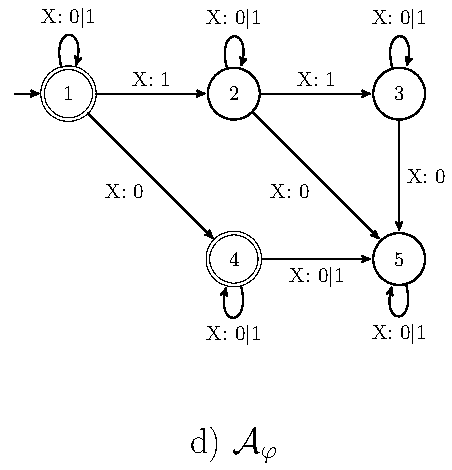
\includegraphics{formula-automaton.pdf}}}
  \only<5>{\scalebox{0.55}{\includegraphics{formula-determinization.pdf}}}
  \only<6-7>{\scalebox{0.55}{\includegraphics{formula-complement.pdf}}}
 \end{center}
\end{figure}
  \end{frame}
  
  \begin{frame}{Srovnání přístupů přes DFA a NFA}
  \begin{itemize}
    \item Proč {\color{red} NEPOUŽÍVAT} deterministické automaty:
    \pause
    \begin{enumerate}
      \item Každá alternace kvantifikátorů přidává úroveň determinizace
      \pause
      \begin{itemize}
        \item[$\Rightarrow$]stavová exploze
      \pause
        \item[$\Rightarrow$]ztráta historie stavů
      \pause
      \end{itemize}
      \item Nutnost implementace heuristik (nástroj MONA)
      \pause
    \end{enumerate}
    \item Proč {\color{green} POUŽÍVAT} nedeterministické automaty:
    \begin{enumerate}
      \pause
      \item Existence knihoven pro efektivní manipulaci s nedeterministickými
      automaty (\texttt{libvata})
      \pause
      \item Výrazný pokrok v algoritmech nad nedeterministickými automaty jako
      např.
      testování jazykové inkluze či universality jazyka automatu
      \begin{itemize}
      \pause
        \item[$\Rightarrow$]algoritmy založené na antichainech
      \end{itemize}
    \end{enumerate}
  \end{itemize}
  \end{frame}
  
  \begin{frame}[t]{Rozhodování WS$k$S pomocí NFA}
  \begin{itemize}
  \item Mějme formuli $\psi$, takovou, že $freeVars(\varphi) = \emptyset$ ve
  tvaru:
  \end{itemize}
  \begin{equation*}
 \psi \overset{\mathit{def}}{=}
 \exists\mathcal{X}_{m}\neg\ldots\neg\exists\mathcal{X}_1: \pi(\mathbb{X}).
\end{equation*}
  \begin{itemize}
    \item Definujeme rodinu hierarchických formulí $\Phi$ a k ní korespondující
    rodinu automatů $\mathbb{A}$ takovou, že:
    \begin{eqnarray}
     \varphi_0 & = & \pi\\
     \varphi_i & = & \neg\exists\mathcal{X}_i\varphi_{i-1}
    \end{eqnarray}
    \item Explicitní konstrukce pouze u automatu $\mathcal{A}_{\varphi_0}$
  \end{itemize}
  
  \end{frame}
  
    \begin{frame}{Rozhodování WS$k$S pomocí NFA: Algoritmus}
  \begin{algorithm}[H]
  \SetAlgorithmName{Algoritmus}{algoritmus}{Seznam algoritmů}
  		\SetKwInput{KwIn}{Vstup}
  		\SetKwInput{KwOut}{Výstup}
		\SetKwFor{For}{foreach}{do}{}
		\SetKwRepeat{Repeat}{repeat}{until}
		\KwIn{Počáteční stav $I_m$ automatu $A_{\varphi_m}$, Automat
		$\mathcal{A}_{\varphi_0}$}
		\KwOut{\textsc{TRUE} pokud stav $I_m$ je koncový, \textsc{FALSE}
		jinak}
		\BlankLine
		\Return IsStateAccepting($I_m$, $m$)\;
		\SetKwProg{myproc}{Funkce}{}{}
		\BlankLine
		  \myproc{IsStateAccepting(state Q, level i)}{
		   \For{$q \in Q$}{
		     \uIf{IsStateAccepting(q, i-1)}{
		       \Return \textsc{FALSE}\;
		       }
		   }
		   \Return IsReachableAccepting(Q, i, $\delta_0^i$)\;
		  }
		\caption{Rozhodování platnosti WS$k$S formule $\psi$}
	\end{algorithm}
  
  \end{frame}
  
  
  \begin{frame}[t]{Demonstrace účinnosti algoritmu}
    \begin{itemize}
    \item[] Mějme formuli $\varphi \overset{\mathit{def}}{=}
    \neg\exists P:
    Singleton(P) \wedge P
    \not\subseteq X$
%      \only<2,3>{\item Je makro-stav $\{\{1\}\}$ {\color{blue} koncový?}
%      }\only<3>{ $\Rightarrow$ Ano, pokud $\exists q \in \{\{1\}\}$ který je
%      koncový} 
%      \only<4,5>{\item Je makro-stav $\{1\}$ {\color{blue} koncový?}
%      } \only<5>{$\Rightarrow$ Ano, pokud $\forall q \in \{1\}$ jsou nekoncové}
%      \only<6,7>{\item Je stav $1$ {\color{blue} koncový?} }
%      \only<7>{$\Rightarrow$ Ano!}
%      \only<8,9>{\item Je makro-stav $\{1\}$ {\color{blue} koncový?}}
%      \only<9>{ $\Rightarrow$ Není!}
%      \only<10>{\item Generujeme následníka $\{\{1\}\}$ a testujeme jeho
%      konečnost}
%      \only<11>{\item Uplatnění antichainů: $\forall q \in \{\{1\}\}: \exists r
%      \in \{\{1, 2\}, \{1, 4\}\}: q \subseteq r$ \pause$\Rightarrow$ Ukončíme
%      prohledávání stavového prostoru.}
	\item Při prohledávání stavového prostoru nemusíme dále prozkoumávat následníky
	počátečního stavu $\{1, 2\}$ a $\{1, 4\}$
    \end{itemize}
    
      \begin{figure}
 \begin{center}
 \scalebox{0.45}{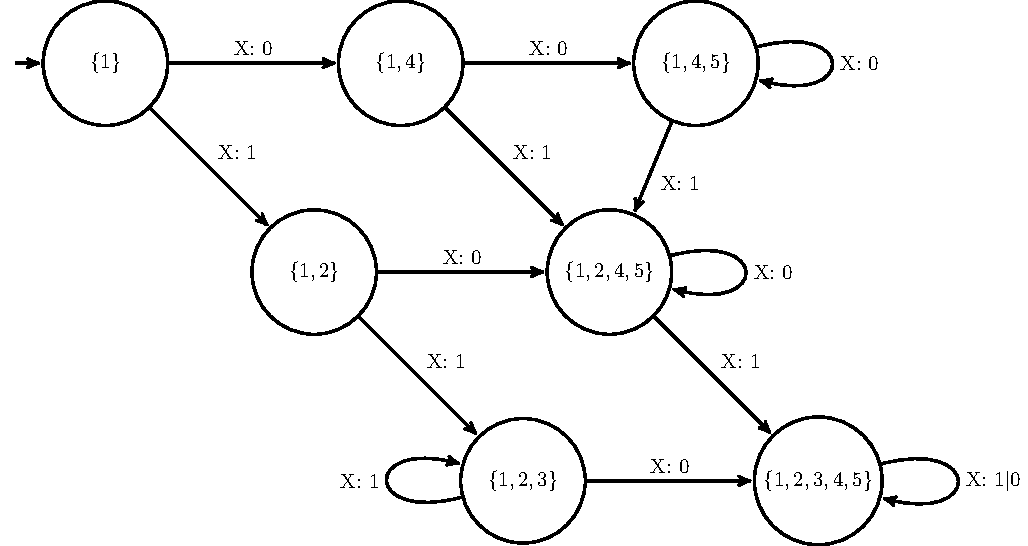
\includegraphics{antichain-meets-projection.pdf}}
 \end{center}
\end{figure}
    
%       \begin{figure}
%  \begin{center}
%   \only<2,3>{\scalebox{0.8}{\includegraphics{formula-step1.pdf}}}
%     \only<4,5,8,9>{\scalebox{0.8}{\includegraphics{formula-step2.pdf}}}
%       \only<6,7>{\scalebox{0.8}{\includegraphics{formula-step3.pdf}}}
%         \only<10,11>{\scalebox{0.8}{\includegraphics{formula-step4.pdf}}}
%  \end{center}
% \end{figure}
  \end{frame}
  
  \begin{frame}{Shrnutí}
  \begin{itemize}
    \item Představen přístup k rozhodování logiky WS$k$S za pomocí použití
    nedeterministických automatů
      \pause
    \item Využití knihovny \texttt{libvata} pro efektivní manipulaci s NTA
      \pause
    \item Aktuální implementace rozhoduje nekvantifikované formule a v omezené
    míře kvantifikované formule bez alternací
      \pause
    \item Velký prostor pro optimalizace
    \begin{itemize}
      \item[$\Rightarrow$]cachování,
      \item[$\Rightarrow$]reprezentace formule pomocí
	    \textcolor{blue}{orientovaných acyklických grafů} (DAG).
    \end{itemize}
  \end{itemize}
  \end{frame}

\end{document}
